
\chapter{Monte-Carlo simulation}\label{chap:MC}
The Monte Carlo (MC) method was invented by scientists working on the atomic bomb in the 1940s. Its core idea is to use random samples of parameters or inputs to explore the behavior of a complex system or process.  Nowadays, MC experiments are essential part of research in both theoretical and experimental particle physics.
This chapter gives an overview of the ATLAS experiment simulation scheme, the simulation methods and the software used. Also, techniques for fast simulation will be discussed. 

\section{\atlas chain of Monte-Carlo production}

\begin{figure}[!b]
\center{
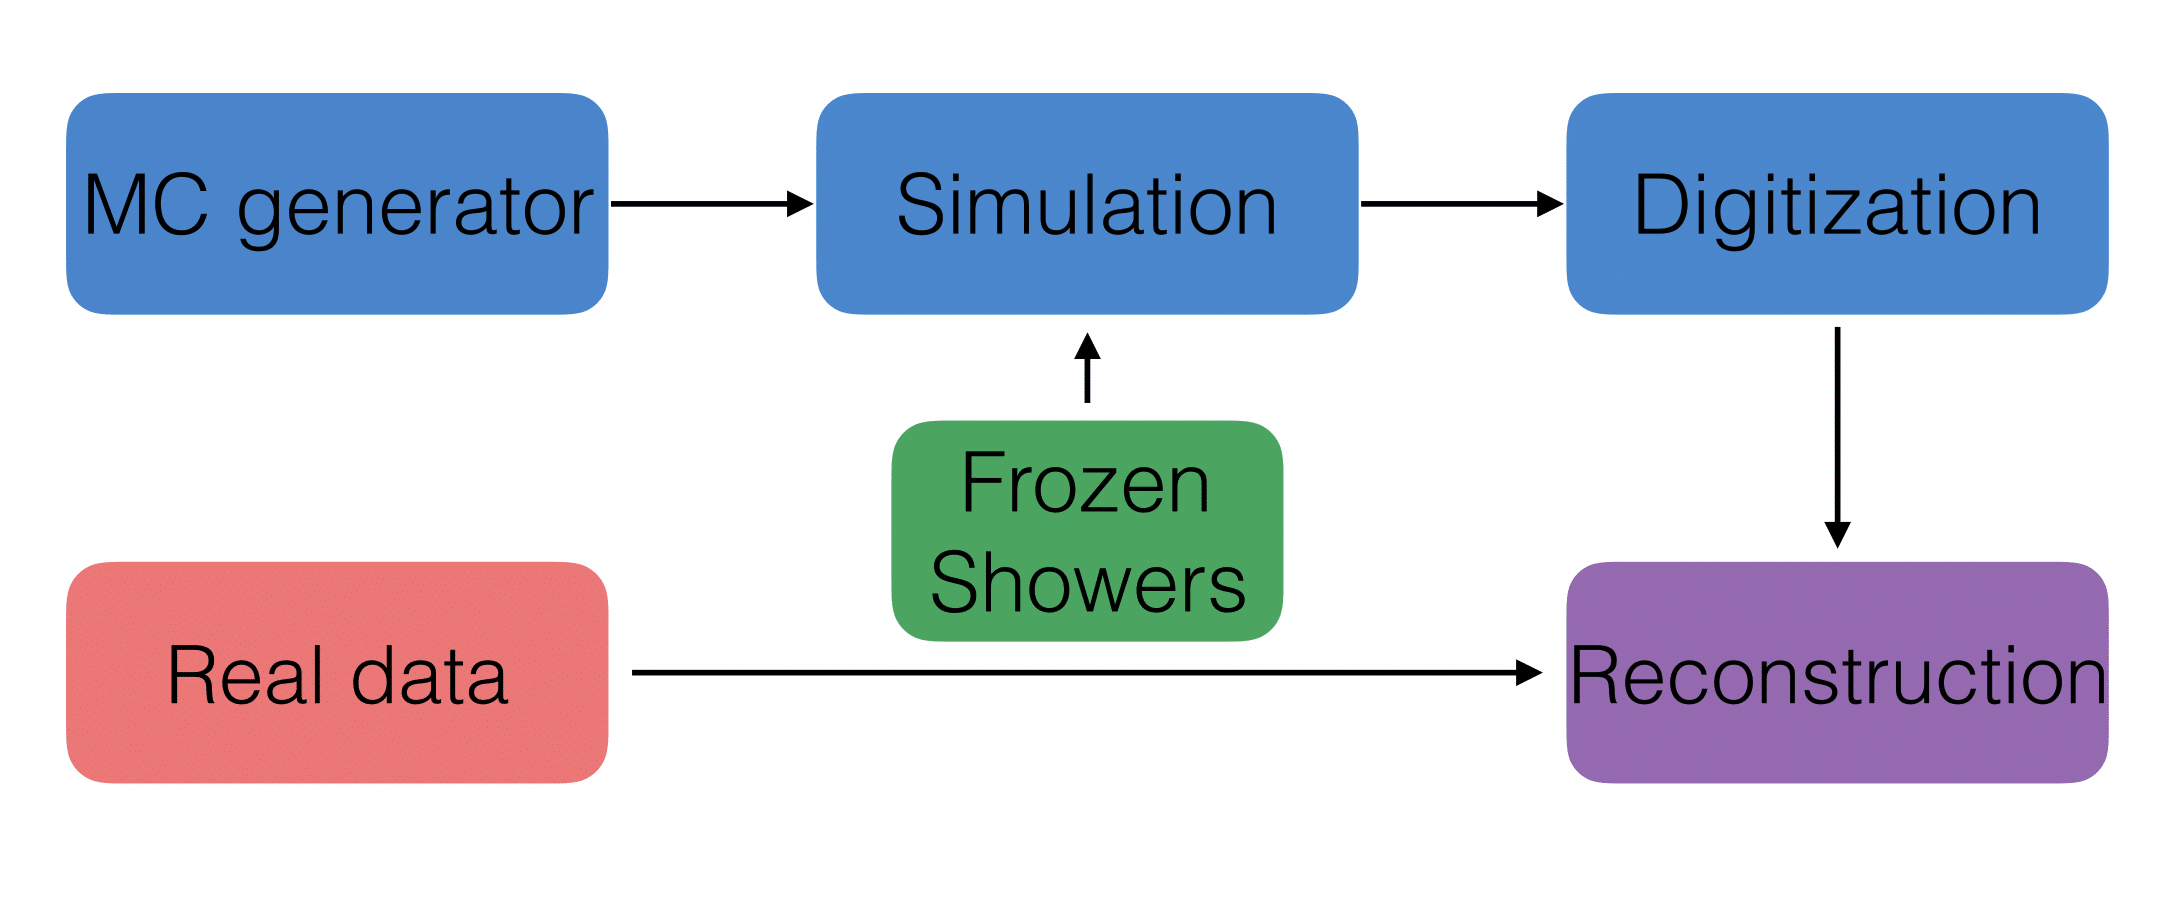
\includegraphics[width=0.6\textwidth]{MC/MCScheme.png}
\caption{Diagram of the \atlas MC production chain. Stages in blue are completelly related to Monte-Carlo production. The Frozen Showers technique for fast simulation will be explained in Chap. \ref{chap:FS}. Data sample collection is decribed in Sec. \ref{sec:ATLAS}. Reconstruction is common stage for data and MC and described in Chap. \ref{chap:Rec}. After the reconstruction events are going to the analysis chain.}
\label{fig:MC_gen2}}
\end{figure}

Monte Carlo method allows to perform different analyses, generate predictions for comparisons with data, study the the detector or the selection algorithms performance. All of these applications require accurate MC predictions. The simulation software implements precise physics models and uses statistics large enough , to exclude statistical uncertainties (usually 5 times more, than expected in a data). \atlas simulation software is integrated into Athena framework. 

Simulation chain is generally divided into 4 main steps (Figure ~\ref{fig:MC_gen2}):
\begin{description}
\item[Event generation]Simulation of hard interaction, partion evolution and hadronisation. This step is independent of the \atlas detector geometry.
\item[Simulation]Simulation of energy depositions ("hits") which are produced by final state particles.
\item[Digitalization] Simulation of detector responce using "hits" information:  first inputs to the read out drivers (ROD's), called "digits" are constructed, then ROD functionality is emulated. Detector noise effects are added at this stage. 
\item[Reconstruction] Production of the Analysis Object Data (AOD) files, which are containing the information needed for physics analysis. This stage is identical for both data and MC
\end{description}
Additionally, the pileup effects are added to MC by overlaying the simulation of the hard interactions with the simulation of soft inelastic scatterings. This scheme allows to use computing resources more efficiently, than with a single-step simulation and simplifies software validation, since it is possible to reuse files from previous stages. In the following sections event generation and simulation will be described in more details.

\section{Event generators}

\begin{figure}[!t]
\begin{center}
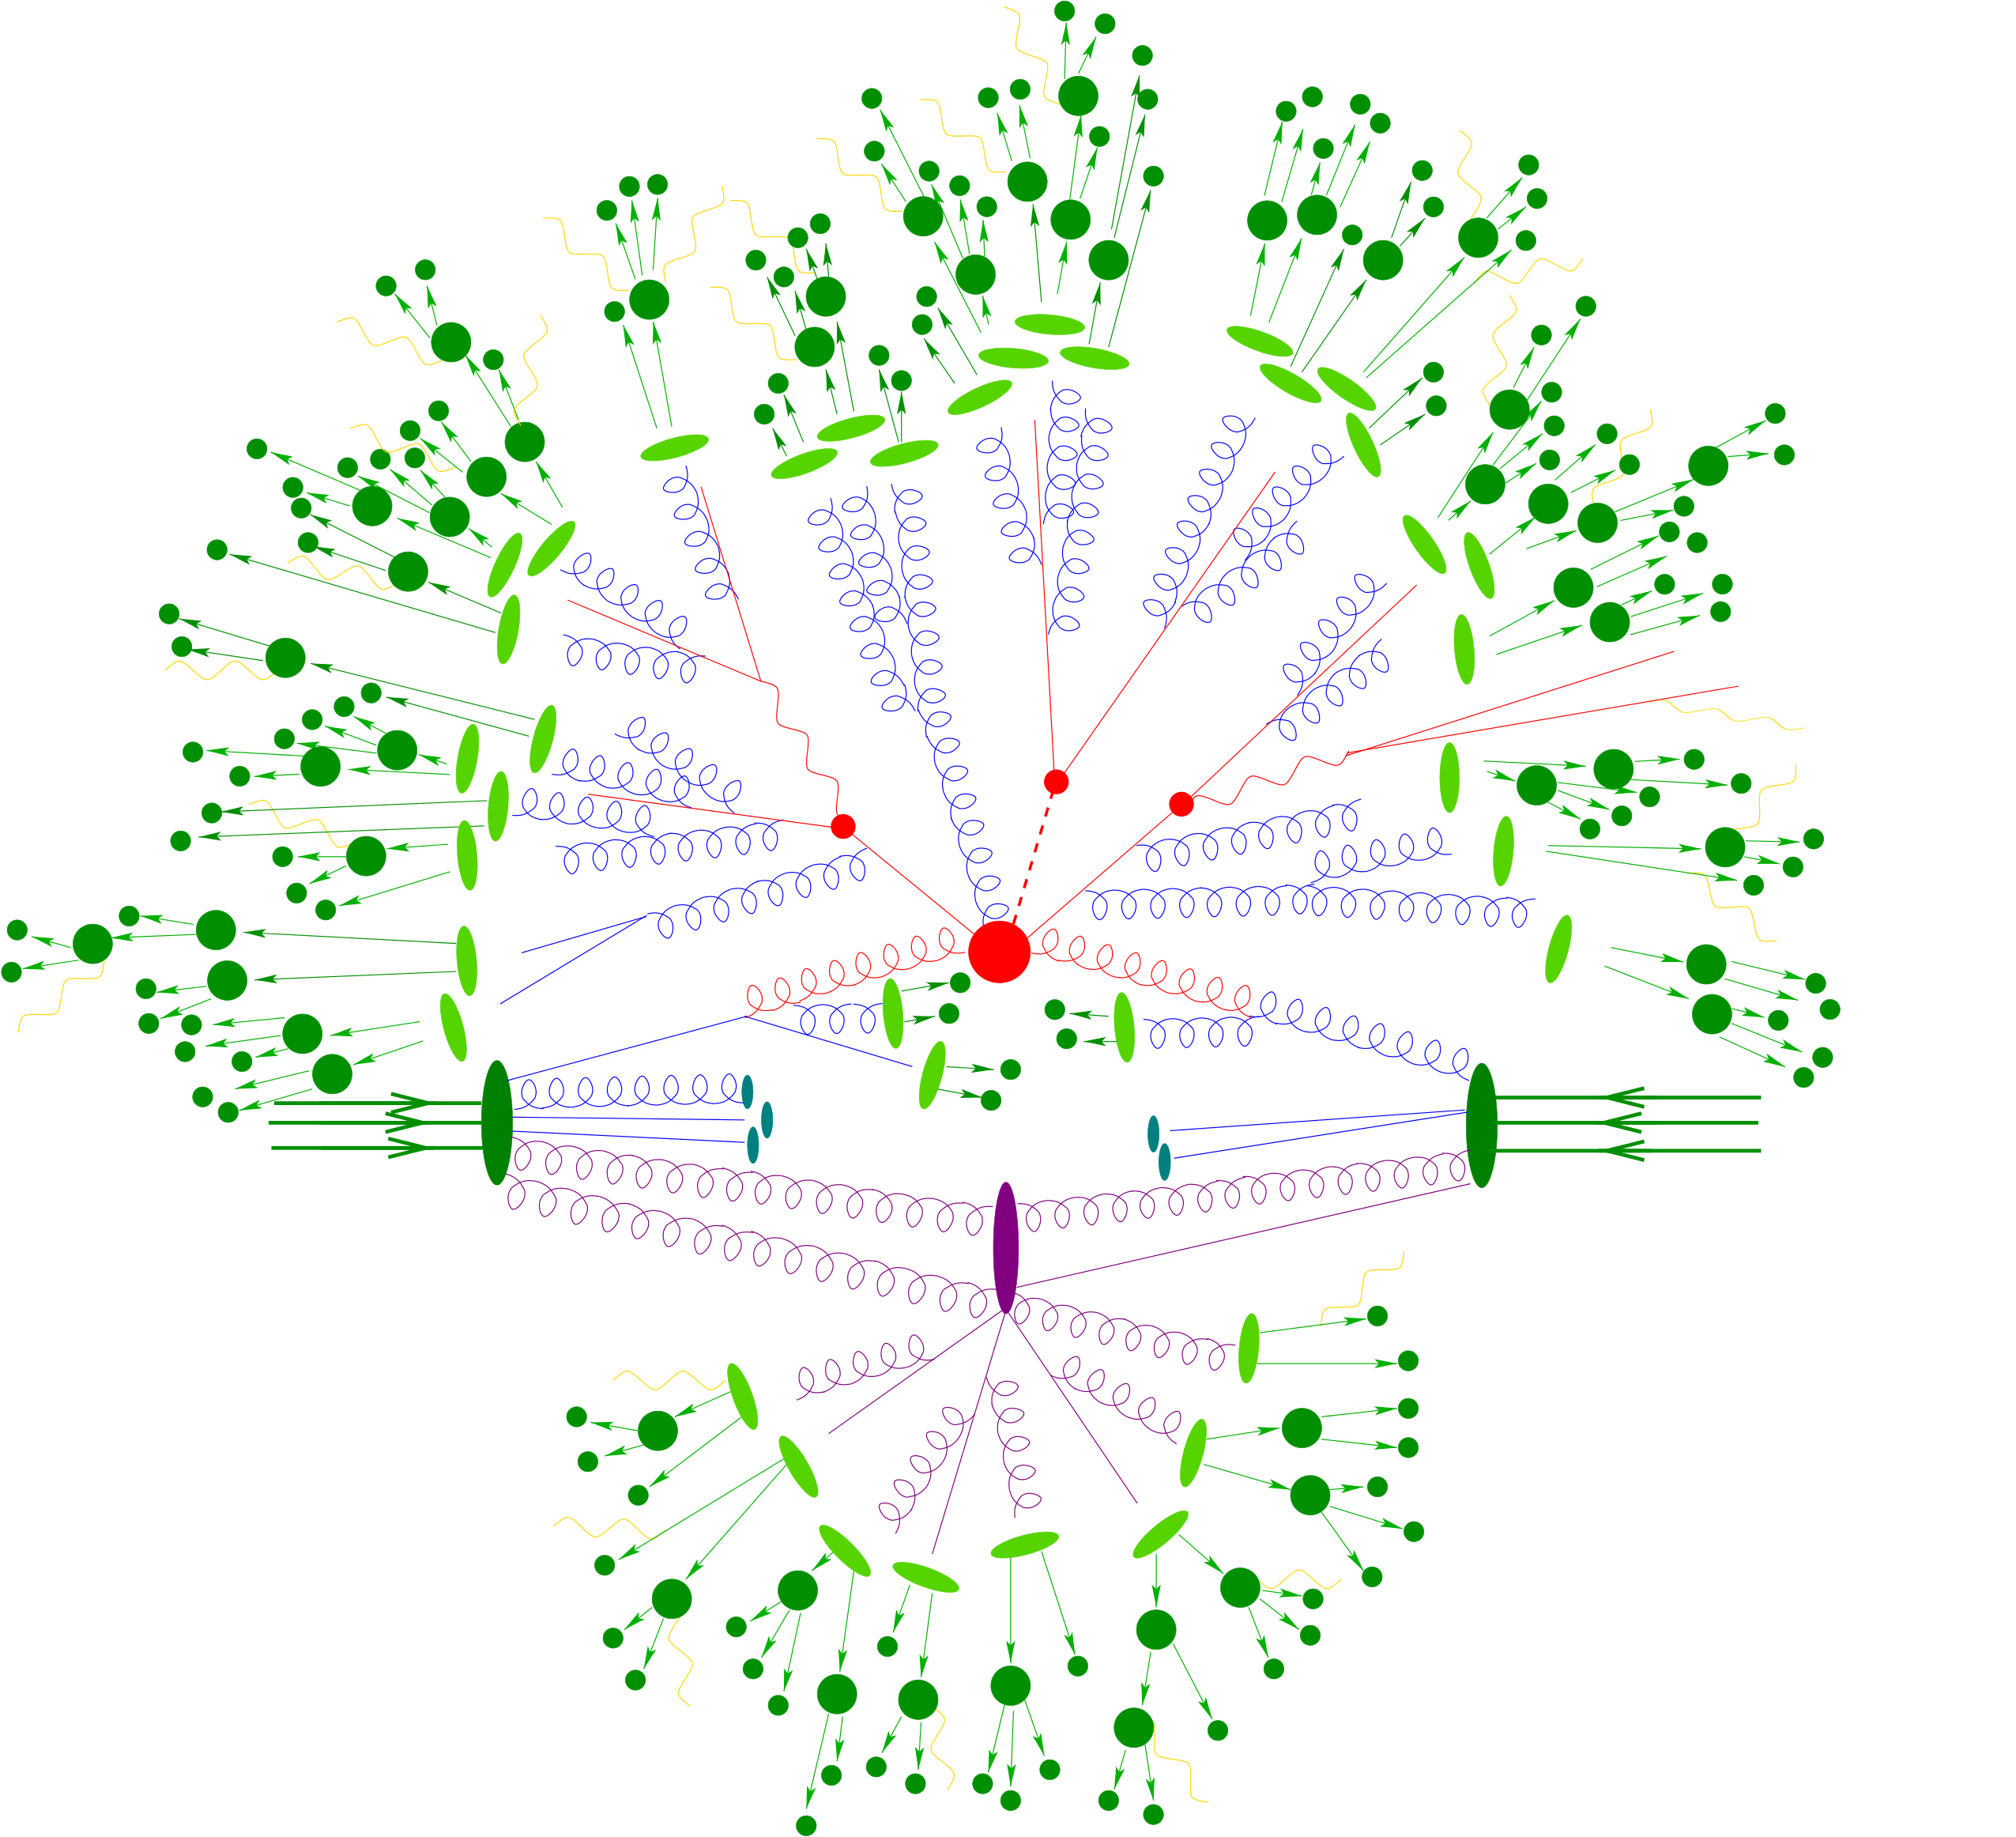
\includegraphics[width=0.5\textwidth]{MC/tth_Event}
\end{center}
\caption{Schematic view of a $t\bar{t}H$ event produced in a pp-collision: the hard scattering is shown as a red blob with the solid and dashed lines as the resulting three particles.
Independently happening multi-particle interactions are indicated by the violet blob. 
Parton showers are shown with curly lines.
Hadronization yields hadrons as shown in light green, while the final state particle are dark green.\cite{MC:ttHSketch}
}
\label{fig:MC_ttH}
\end{figure}

The outcome of the hard interaction could be a simple scattering of the hadron elementary constituents, their annihilation into new resonances or a combination of two. This can lead to a final state with a large particle multiplicity. The main goal of the event generator is to provide a complete picture of the final state: description of the particle types and momentia on  the event-by-event basis. The factorisation theorem \cite{Factorisation} allows to make event generation in independent stages, which are dominated by different dynamics. Schematic plan of simulation of a $t\bar{t}H$ event is shown in Figure \ref{fig:MC_ttH}:

\begin{description}

\item[Modelling of hard subprocess] Hard subprocess happens at the smallest times and distances, where the colliding partons are considered free. The process of interest is simulated by selecting production channels and calculating corresponding matrix elements (ME)  at a fixed order of the strong coupling constant and including randomly chosen momenta of the incoming partons, which are based on the parton distribution functions (PDF). Most of the generators have leading (LO) order or next to leading order (NLO) in $\alpha_s$. 
\item[Parton showering] Quarks and gluons from hard process can radiate secondary quarks and gluons, resulting in dozens of additional partons associated with the event. This process is calculated as step-by-step evolution of momentum transfer scales from highest (hard subprocess), to the lowest (around 1 GeV), where the pertrubative calculations are not valid. 
There is a possiblity of double counting between showers and hard subprocess. This can be avoided using matching approaches, for which higher order corrections to ME are integrated with parton showers, or merging strategy, there jet resolution scale is used as an threshold between matrix elements and parton showers. 
\item[Hadronisation] Final, stable, color-neutral particles, which can be detected in an experiment, are formed during hadronisation. This occures at larger nonpertrubative scales and  is usually implemented using different phenomenological models.
\item[Modelling underlying event] Parallel to the main process other collisions of partons can occur. They are called underlying event. These additional interaction can produce partons which contribute to the final state. This is one of the least understood aspect of hadronic collisions. 

\end{description}


The current analysis uses samples generated with the following generators:
\begin{itemize}[align=left]
\item[Powheg \cite{Powheg}] Powheg is Monte-Carlo, which calculates the matrix element (ME) at the NLO level \cite{PowhegNLO}, that can be interfaced to other generators (such as Pythia or Herwig) to get higher precision of showering.
\item[Pythia \cite{Pythia6}] Pythia is a general purpose generator for hadronic, hadron-lepton and leptonic collisions. It can model ME, initial and final state showers, hadronisation and decays, underlying event (via multi parton interactions). Pythia contains library with around 240 processes with LO ME. It uses Lund String model \cite{LundString} for hadronisation.
\item[Herwig \cite{Herwig}] Herwig is a LO general purpose event generator for simulation of lepton-lepton, hadron-lepton and hadron-hadron collisitons. The main difference between Pythia and Herwig is that Herwig uses angular ordering in the parton showers and models the hadronisation step using the cluster fragmentation
\item[Sherpa \cite{Sherpa}] Sherpa is an event generator, that uses tree-level leading order matrix element for a hard scattering and features its own implementation of parton shower and hadronisation models.
\item[Photos \cite{Photos}] Photos is a program used for generation of QED radiative corrections. It is linked to multipurpose generators.
\item[Tauola \cite{taluola}] Tauola is a generator, used to describe leptonic and semi-leptonic $\tau$-decays. It is also linked to multipurpose generators.
\end{itemize}

\section{Simulation in Geant4}

After event generation, simulation software is used to provide hardware response for final state particles. The main method used by \atlas experiment, referred to as \textit{Full Simulation}, makes use of the Geant4\cite{Geant4}. Geant4 is C++ based toolkit for the simulation of the passage of particles through matter. It is used in a wide range of experiments in high energy and nuclear physics.

Geant4 can simulate complex detector structures with sensitive detector material and corresponding infrastructure. It can also calculate basic properties of materials, like radiation and interaction length. Geant4 stores "hits" information  - snapshots of physical interactions. 
In Geant4 events and particles are simulated separately and each particle is moved in steps. Size of each step is chosen to preserve both CPU performance and required precision. 

Physics interactions are treated as a set of discrete processes. They could be handled either for particle at rest, or its along step, the maximum value of which depends on physics process, or after it. Geant4 package has different models and approximations for hadronic and electromagnetic processes. Some of them are approximate and computationally fast. It allows to choose a set of the models, called physics list, depending on particular requirements. There are several reference physics lists, that are validated for each new release of Geant4 software. \atlas experiment uses one of these lists.

Most of the computing resources are taken by a mass MC production, required for each data taking periods. Uncertainties of some of Run-I analyses are dominated by available MC statistics. It is possible to improve in CPU usage by tuning physics list or replacing a complex magnetic field maps by a parametrisation. Also there are long-term developments for multi-threading and vectorisation of the code. 

Run-2 has a higher pileup and luminosity, so even more MC events are needed. This means that fast and accurate simulation approach is essential. During the simulation largest time is spent on calorimeters. This is the motivation for development of fast calorimetry techniques.  

There are two main methods used at \atlas:
\begin{itemize}
\item Parametrisation of the calorimeter cells response. Spacial energy response is simulated using longitudial and lateral energy profiles.
\item Frozen Showers. This technique will be described in more detailed in Chap. \ref{chap:FS}
\end{itemize}

